\documentclass[10pt]{article}
\usepackage[margin=0.55in,includeheadfoot]{geometry}
\usepackage[T1]{fontenc}
\usepackage[utf8]{inputenc}
\usepackage{lmodern}
\usepackage{multicol}
\usepackage{enumitem}
\usepackage{booktabs}
\usepackage{array}
\usepackage{amsmath,amssymb}
\usepackage{tikz}
\usepackage{graphicx}
\usepackage{eso-pic}
\usepackage{fancyhdr}
\usepackage{lastpage}
\usepackage{needspace}
\usepackage{xcolor}
\usepackage[hidelinks]{hyperref}
\setlength{\columnsep}{0.28in}
\setlength{\parindent}{0pt}
\setlength{\parskip}{0.35em}
\emergencystretch=1em
\raggedbottom
\pagestyle{fancy}
\fancyhf{}
\fancyhead[L]{\textsf{AP MICROECONOMICS}}
\fancyhead[C]{\textsf{Curve Challenge Booklet}}
\fancyhead[R]{\textsf{Page \thepage\ of \pageref*{LastPage}}}
\fancyfoot[R]{\textsf{GO TO THE NEXT PAGE.}}
\renewcommand{\headrulewidth}{0.4pt}
\renewcommand{\footrulewidth}{0pt}
\newenvironment{choiceslist}
  {\begin{enumerate}[label=(\Alph*), leftmargin=1.55em, itemsep=0.1em, topsep=0.15em, parsep=0pt]}
  {\end{enumerate}}
\newenvironment{stimulus}
  {\begin{center}\begin{minipage}{0.97\columnwidth}\footnotesize\itshape\setlength{\tabcolsep}{3pt}\renewcommand{\arraystretch}{0.96}}
  {\end{minipage}\end{center}}
\newcommand{\sectiontitle}[1]{%
  \vspace{0.35em}
  {\large\bfseries #1\par}
  \vspace{0.15em}
  \hrule
  \vspace{0.4em}
}
\newcommand{\CodexWatermark}{%
  \AddToShipoutPictureBG{%
    \AtPageCenter{%
      \makebox(0,0){%
        \rotatebox{45}{%
          \textcolor[gray]{0.93}{\fontsize{22}{22}\selectfont\bfseries Winston Huang-Generated with Codex}%
        }%
      }%
    }%
  }%
}
\begin{document}
\CodexWatermark
{\centering
{\LARGE\bfseries AP Microeconomics Curve Challenge\par}
\vspace{0.35em}
{\large 40 Hard AP-Style Graph and Curve Problems\par}
\vspace{0.85em}}
\textbf{Directions:} Choose the best answer for each question. Every question in this booklet is built around a graph, curve, or curve-based inference in the style of difficult AP Microeconomics multiple-choice and FRQ graph reasoning.

\textbf{Source basis:} The topics, graph types, and traps in this booklet were synthesized from the 82 TB/SG/FRQ/progress-check PDFs in this folder, especially the repeated graph work on price controls, taxation, trade, perfect competition, monopoly, monopolistic competition, labor markets, monopsony, externalities, and inequality.

\vspace{0.7em}
\begin{multicols*}{2}
\sectiontitle{Graph Problems}
\Needspace{18\baselineskip}
\begin{stimulus}
The following questions refer to the graph below, which shows the market for tickets to an annual event with a fixed seating capacity.

\begin{center}
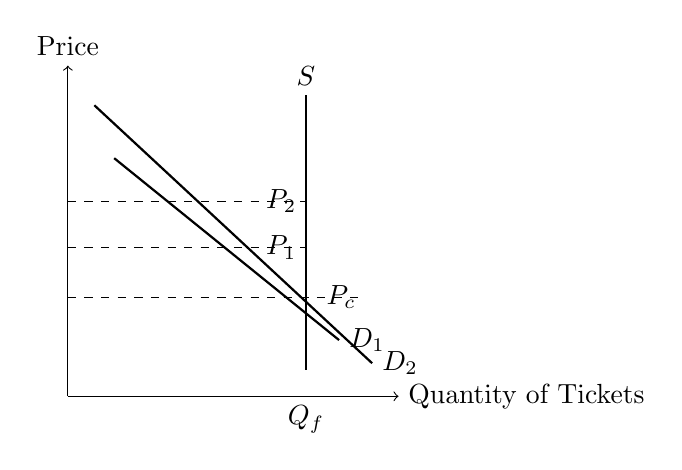
\begin{tikzpicture}[x=0.42cm,y=0.42cm]
\draw[->] (0,0) -- (10,0) node[right] {Quantity of Tickets};
\draw[->] (0,0) -- (0,10) node[above] {Price};
\draw[thick] (7.2,0.8) -- (7.2,9.1) node[above] {$S$};
\draw[thick] (0.8,8.8) -- (9.2,1.0) node[right] {$D_2$};
\draw[thick] (1.4,7.2) -- (8.2,1.7) node[right] {$D_1$};
\draw[dashed] (0,4.5) -- (7.2,4.5) node[left] {$P_1$};
\draw[dashed] (0,5.9) -- (7.2,5.9) node[left] {$P_2$};
\draw[dashed] (0,3.0) -- (9.0,3.0) node[left] {$P_c$};
\node[below] at (7.2,0) {$Q_f$};
\end{tikzpicture}
\end{center}
\end{stimulus}
\begin{enumerate}[series=curveq, leftmargin=*, itemsep=0.8em, topsep=0.18em, parsep=0pt]
\item If demand shifts from $D_1$ to $D_2$ and no price ceiling is imposed, which of the following will occur?
\begin{choiceslist}
\item Price will remain at $P_1$ and quantity will remain at $Q_f$.
\item Price will rise to $P_2$ and quantity will increase beyond $Q_f$.
\item Price will rise to $P_2$ and quantity will remain at $Q_f$.
\item Price will fall to $P_c$ and quantity will remain at $Q_f$.
\item Price will rise to $P_2$ and quantity will fall below $Q_f$.
\end{choiceslist}
\item Suppose a binding price ceiling is set at $P_c$ after demand has shifted to $D_2$. The market outcome will most likely be
\begin{choiceslist}
\item quantity exchanged greater than $Q_f$ because the lower price stimulates more demand
\item quantity exchanged equal to $Q_f$ with a shortage because quantity demanded at $P_c$ exceeds quantity supplied
\item quantity exchanged less than $Q_f$ because suppliers reduce output when price falls
\item quantity exchanged equal to the quantity demanded on $D_2$ at $P_c$
\item no shortage because the original supply is vertical
\end{choiceslist}
\item Relative to the original equilibrium with demand curve $D_1$, the event organizer's total revenue after the shift to $D_2$ and with no price ceiling will
\begin{choiceslist}
\item increase because the same number of tickets is sold at a higher price
\item decrease because demand becomes less elastic near the top of the graph
\item remain unchanged because quantity is fixed
\item decrease because a vertical supply curve prevents market adjustment
\item be indeterminate because elasticity is not labeled numerically
\end{choiceslist}
\item If the binding ceiling at $P_c$ remains in place and resale is possible, which of the following is most accurate?
\begin{choiceslist}
\item All buyers will necessarily pay exactly $P_c$ because the law fixes the final transaction price.
\item No resale can occur because quantity supplied is perfectly inelastic.
\item Producer surplus must rise because the event remains sold out.
\item Some buyers may end up paying more than $P_c$ in a secondary market.
\item The shortage disappears once buyers understand the supply curve is vertical.
\end{choiceslist}
\end{enumerate}
\Needspace{18\baselineskip}
\begin{stimulus}
The following questions refer to the graph below, which shows a small country that imports a good at world price $P_w$. Afterward, the country imposes a tariff that raises the domestic price to $P_t$.

\begin{center}
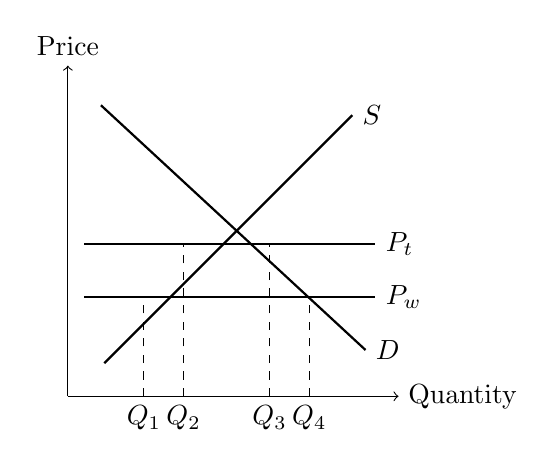
\begin{tikzpicture}[x=0.42cm,y=0.42cm]
\draw[->] (0,0) -- (10,0) node[right] {Quantity};
\draw[->] (0,0) -- (0,10) node[above] {Price};
\draw[thick] (1.0,8.8) -- (9.0,1.4) node[right] {$D$};
\draw[thick] (1.1,1.0) -- (8.6,8.5) node[right] {$S$};
\draw[thick] (0.5,3.0) -- (9.3,3.0) node[right] {$P_w$};
\draw[thick] (0.5,4.6) -- (9.3,4.6) node[right] {$P_t$};
\draw[dashed] (2.3,0) -- (2.3,3.0);
\draw[dashed] (3.5,0) -- (3.5,4.6);
\draw[dashed] (6.1,0) -- (6.1,4.6);
\draw[dashed] (7.3,0) -- (7.3,3.0);
\node[below] at (2.3,0) {$Q_1$};
\node[below] at (3.5,0) {$Q_2$};
\node[below] at (6.1,0) {$Q_3$};
\node[below] at (7.3,0) {$Q_4$};
\end{tikzpicture}
\end{center}
\end{stimulus}
\begin{enumerate}[resume*=curveq, leftmargin=*, itemsep=0.8em, topsep=0.18em, parsep=0pt]
\item Before the tariff is imposed, the quantity imported by the country is
\begin{choiceslist}
\item $Q_2-Q_1$
\item $Q_3-Q_2$
\item $Q_4-Q_3$
\item $Q_4-Q_2$
\item $Q_4-Q_1$
\end{choiceslist}
\item After the tariff is imposed and the domestic price rises to $P_t$, the quantity imported becomes
\begin{choiceslist}
\item $Q_2-Q_1$
\item $Q_3-Q_2$
\item $Q_4-Q_3$
\item $Q_4-Q_1$
\item $Q_3-Q_1$
\end{choiceslist}
\item Which of the following expressions gives the government's tariff revenue?
\begin{choiceslist}
\item $(P_t-P_w)(Q_4-Q_1)$
\item $(P_t-P_w)(Q_3-Q_2)$
\item $(P_t-P_w)(Q_2-Q_1)$
\item $\tfrac{1}{2}(P_t-P_w)(Q_3-Q_2)$
\item $\tfrac{1}{2}(P_t-P_w)(Q_4-Q_1)$
\end{choiceslist}
\item Relative to free trade, which of the following groups are guaranteed to gain from the tariff?
\begin{choiceslist}
\item Domestic consumers only
\item Domestic producers only
\item Domestic producers and the government
\item Foreign producers and domestic consumers
\item Domestic consumers and the government
\end{choiceslist}
\end{enumerate}
\Needspace{18\baselineskip}
\begin{stimulus}
The following questions refer to the graph below, which shows a competitive market before and after a per-unit excise tax is imposed.

\begin{center}
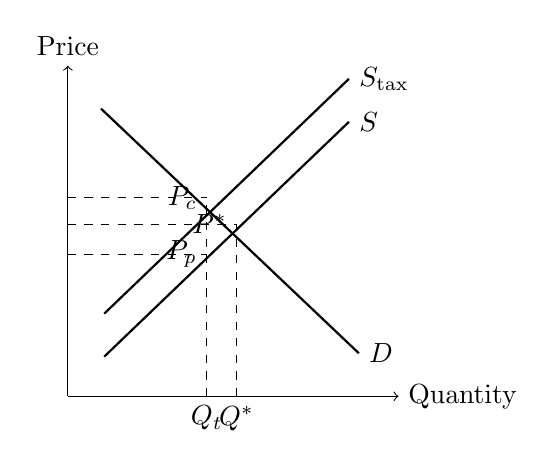
\begin{tikzpicture}[x=0.42cm,y=0.42cm]
\draw[->] (0,0) -- (10,0) node[right] {Quantity};
\draw[->] (0,0) -- (0,10) node[above] {Price};
\draw[thick] (1.0,8.7) -- (8.8,1.3) node[right] {$D$};
\draw[thick] (1.1,1.2) -- (8.5,8.3) node[right] {$S$};
\draw[thick] (1.1,2.5) -- (8.5,9.6) node[right] {$S_{\text{tax}}$};
\draw[dashed] (0,5.2) -- (5.1,5.2) node[left] {$P^{*}$};
\draw[dashed] (0,6.0) -- (4.2,6.0) node[left] {$P_c$};
\draw[dashed] (0,4.3) -- (4.2,4.3) node[left] {$P_p$};
\draw[dashed] (5.1,0) -- (5.1,5.2);
\draw[dashed] (4.2,0) -- (4.2,6.0);
\node[below] at (5.1,0) {$Q^{*}$};
\node[below] at (4.2,0) {$Q_t$};
\end{tikzpicture}
\end{center}
\end{stimulus}
\begin{enumerate}[resume*=curveq, leftmargin=*, itemsep=0.8em, topsep=0.18em, parsep=0pt]
\item Based on the graph, the larger share of the tax burden is borne by
\begin{choiceslist}
\item consumers, because the increase from $P^{*}$ to $P_c$ is larger than the decrease from $P^{*}$ to $P_p$
\item producers, because the tax is legally imposed on sellers
\item consumers and producers equally, because the tax wedge is fixed
\item the government, because quantity falls from $Q^{*}$ to $Q_t$
\item consumers, but only if demand is perfectly inelastic
\end{choiceslist}
\item Which of the following expressions equals total tax revenue after the tax is imposed?
\begin{choiceslist}
\item $(P_c-P^{*})Q^{*}$
\item $(P^{*}-P_p)Q^{*}$
\item $(P_c-P_p)Q_t$
\item $\tfrac{1}{2}(P_c-P_p)Q_t$
\item $(P_c-P_p)(Q^{*}-Q_t)$
\end{choiceslist}
\item The deadweight loss created by the tax is measured by
\begin{choiceslist}
\item $\tfrac{1}{2}(P_c-P_p)(Q^{*}-Q_t)$
\item $(P_c-P_p)Q_t$
\item $\tfrac{1}{2}(P_c-P^{*})Q_t$
\item $(P^{*}-P_p)(Q^{*}-Q_t)$
\item $(P_c-P_p)Q^{*}$
\end{choiceslist}
\item If supply became more elastic while demand remained unchanged, which of the following would most likely occur?
\begin{choiceslist}
\item Consumers would bear a larger share of the tax burden.
\item Producers would bear a larger share of the tax burden.
\item Consumers and producers would still bear equal shares.
\item Tax revenue would necessarily rise.
\item Deadweight loss would necessarily fall to zero.
\end{choiceslist}
\end{enumerate}
\Needspace{18\baselineskip}
\begin{stimulus}
The following questions refer to the graph below, which shows a perfectly competitive firm's short-run cost curves and two possible market prices.

\begin{center}
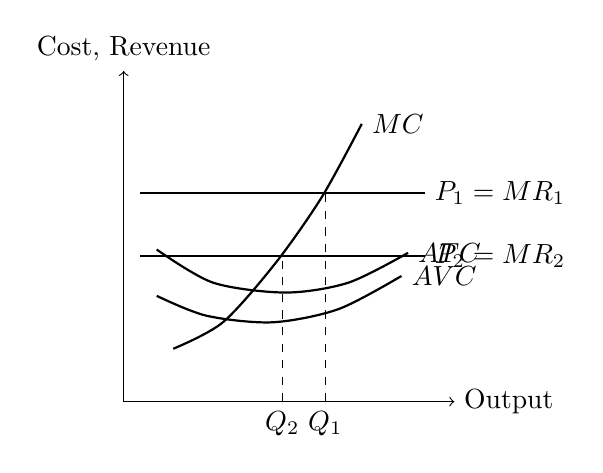
\begin{tikzpicture}[x=0.42cm,y=0.42cm]
\draw[->] (0,0) -- (10,0) node[right] {Output};
\draw[->] (0,0) -- (0,10) node[above] {Cost, Revenue};
\draw[thick] plot[smooth] coordinates {(1.0,3.2) (2.5,2.6) (4.5,2.4) (6.5,2.8) (8.4,3.8)} node[right] {$AVC$};
\draw[thick] plot[smooth] coordinates {(1.0,4.6) (2.7,3.6) (4.9,3.3) (6.8,3.6) (8.6,4.5)} node[right] {$ATC$};
\draw[thick] plot[smooth] coordinates {(1.5,1.6) (3.0,2.4) (4.6,4.2) (6.0,6.2) (7.2,8.4)} node[right] {$MC$};
\draw[thick] (0.5,6.3) -- (9.1,6.3) node[right] {$P_1=MR_1$};
\draw[thick] (0.5,4.4) -- (9.1,4.4) node[right] {$P_2=MR_2$};
\draw[dashed] (6.1,0) -- (6.1,6.3);
\draw[dashed] (4.8,0) -- (4.8,4.4);
\node[below] at (6.1,0) {$Q_1$};
\node[below] at (4.8,0) {$Q_2$};
\end{tikzpicture}
\end{center}
\end{stimulus}
\begin{enumerate}[resume*=curveq, leftmargin=*, itemsep=0.8em, topsep=0.18em, parsep=0pt]
\item At price $P_1$, the firm's profit-maximizing output and profit situation are
\begin{choiceslist}
\item $Q_1$ and positive economic profit
\item $Q_1$ and negative economic profit
\item $Q_2$ and positive economic profit
\item $Q_2$ and zero economic profit
\item zero output and negative economic profit
\end{choiceslist}
\item At price $P_2$, the firm should
\begin{choiceslist}
\item shut down immediately because $P_2$ is below average total cost
\item produce $Q_2$ because $P_2$ is above AVC even though the firm incurs a loss
\item produce $Q_1$ to spread fixed costs over more output
\item shut down because $P_2$ is below marginal cost at every output
\item produce where ATC is minimized rather than where $P_2=MC$
\end{choiceslist}
\item If the firm's fixed cost increases while the market price remains at $P_2$, the firm's short-run profit-maximizing output will
\begin{choiceslist}
\item rise above $Q_2$
\item fall below $Q_2$
\item remain at $Q_2$
\item fall to zero because ATC shifts up
\item become indeterminate because MC also shifts upward
\end{choiceslist}
\item If many identical firms in the industry are currently earning the same type of profit shown at $P_1$, the most likely long-run market adjustment is that
\begin{choiceslist}
\item market supply will decrease and the price will rise
\item market supply will increase and the price will fall
\item market demand will decrease and the price will rise
\item firms will exit until price rises above $P_1$
\item the long-run equilibrium price will remain at $P_1$ because firms are price takers
\end{choiceslist}
\end{enumerate}
\Needspace{18\baselineskip}
\begin{stimulus}
The following questions refer to the graph below, which shows a single-price monopoly.

\begin{center}
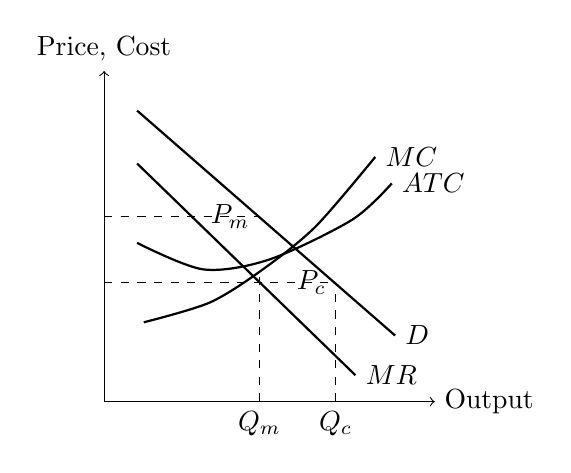
\begin{tikzpicture}[x=0.42cm,y=0.42cm]
\draw[->] (0,0) -- (10,0) node[right] {Output};
\draw[->] (0,0) -- (0,10) node[above] {Price, Cost};
\draw[thick] (1.0,8.8) -- (8.8,2.0) node[right] {$D$};
\draw[thick] (1.0,7.2) -- (7.6,0.8) node[right] {$MR$};
\draw[thick] plot[smooth] coordinates {(1.0,4.8) (3.0,4.0) (5.0,4.3) (7.5,5.5) (8.7,6.6)} node[right] {$ATC$};
\draw[thick] plot[smooth] coordinates {(1.2,2.4) (3.2,3.0) (4.8,4.0) (6.4,5.3) (8.2,7.4)} node[right] {$MC$};
\draw[dashed] (4.7,0) -- (4.7,4.0);
\draw[dashed] (7.0,0) -- (7.0,3.6);
\draw[dashed] (0,5.6) -- (4.7,5.6) node[left] {$P_m$};
\draw[dashed] (0,3.6) -- (7.0,3.6) node[left] {$P_c$};
\node[below] at (4.7,0) {$Q_m$};
\node[below] at (7.0,0) {$Q_c$};
\end{tikzpicture}
\end{center}
\end{stimulus}
\begin{enumerate}[resume*=curveq, leftmargin=*, itemsep=0.8em, topsep=0.18em, parsep=0pt]
\item The monopoly's profit-maximizing output and price are
\begin{choiceslist}
\item $Q_c$ and $P_c$
\item $Q_m$ and $P_m$
\item $Q_m$ and $P_c$
\item $Q_c$ and $P_m$
\item the quantity where $D$ intersects $ATC$ and the price at $MC$
\end{choiceslist}
\item Relative to the allocatively efficient outcome, the unregulated monopoly
\begin{choiceslist}
\item produces too much because $P_m$ exceeds $ATC$
\item produces too little because at $Q_m$, price exceeds marginal cost
\item produces the efficient quantity because $MR=MC$
\item produces the efficient quantity because $P_c=MC$
\item must be productively efficient because it is a single seller
\end{choiceslist}
\item If the monopolist could engage in perfect price discrimination, the quantity produced would most likely
\begin{choiceslist}
\item remain at $Q_m$ because marginal cost is unchanged
\item fall below $Q_m$ because some consumers would pay more
\item rise to $Q_c$, the same quantity a perfectly competitive market would produce
\item rise above $Q_c$ because all consumer surplus is captured
\item become indeterminate because marginal revenue is no longer defined
\end{choiceslist}
\item If regulators force this monopoly to charge a price equal to average total cost, the resulting output will most likely be
\begin{choiceslist}
\item less than $Q_m$
\item equal to $Q_m$
\item between $Q_m$ and $Q_c$
\item equal to $Q_c$
\item greater than $Q_c$
\end{choiceslist}
\end{enumerate}
\Needspace{18\baselineskip}
\begin{stimulus}
The following questions refer to the graph below, which shows a monopolistically competitive firm in long-run equilibrium.

\begin{center}
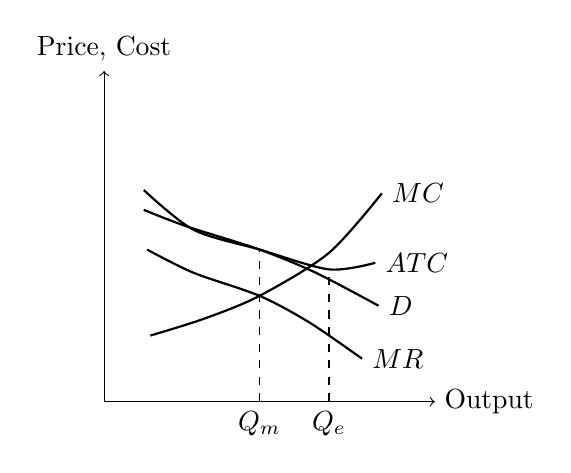
\begin{tikzpicture}[x=0.42cm,y=0.42cm]
\draw[->] (0,0) -- (10,0) node[right] {Output};
\draw[->] (0,0) -- (0,10) node[above] {Price, Cost};
\draw[thick] plot[smooth] coordinates {(1.2,5.8) (2.5,5.3) (4.7,4.6) (6.4,3.9) (8.3,2.9)} node[right] {$D$};
\draw[thick] plot[smooth] coordinates {(1.3,4.6) (2.7,3.9) (4.7,3.2) (6.2,2.4) (7.8,1.3)} node[right] {$MR$};
\draw[thick] plot[smooth] coordinates {(1.2,6.4) (2.7,5.2) (4.7,4.6) (6.8,4.0) (8.2,4.2)} node[right] {$ATC$};
\draw[thick] plot[smooth] coordinates {(1.4,2.0) (3.0,2.5) (4.7,3.2) (6.8,4.5) (8.4,6.3)} node[right] {$MC$};
\draw[dashed] (4.7,0) -- (4.7,4.6);
\draw[dashed] (6.8,0) -- (6.8,4.0);
\node[below] at (4.7,0) {$Q_m$};
\node[below] at (6.8,0) {$Q_e$};
\end{tikzpicture}
\end{center}
\end{stimulus}
\begin{enumerate}[resume*=curveq, leftmargin=*, itemsep=0.8em, topsep=0.18em, parsep=0pt]
\item The graph implies that the firm is earning
\begin{choiceslist}
\item positive economic profit because the demand curve lies above marginal revenue
\item zero economic profit because the demand curve is tangent to the ATC curve at the profit-maximizing quantity
\item negative economic profit because the MC curve is rising
\item normal accounting profit only if price equals marginal cost
\item a loss because output is not at the minimum point of ATC
\end{choiceslist}
\item The firm has excess capacity because
\begin{choiceslist}
\item $Q_m$ is greater than the quantity that minimizes ATC
\item $Q_m$ is less than the quantity that minimizes ATC, labeled $Q_e$
\item the marginal revenue curve lies below the demand curve
\item price exceeds marginal cost
\item its demand curve is downward sloping
\end{choiceslist}
\item Which of the following best describes the firm's allocative efficiency?
\begin{choiceslist}
\item It is allocatively efficient because demand is tangent to ATC.
\item It is allocatively efficient because $MR=MC$ at $Q_m$.
\item It is not allocatively efficient because price exceeds marginal cost at $Q_m$.
\item It is not allocatively efficient because ATC exceeds AVC at all outputs.
\item It is allocatively efficient only if the firm advertises more.
\end{choiceslist}
\item If the firm were instead earning positive economic profit in the short run, the long-run adjustment that would move the firm toward the graph shown is
\begin{choiceslist}
\item entry of new firms that shifts this firm's demand curve leftward
\item exit of firms that shifts this firm's demand curve rightward
\item a decrease in fixed cost that shifts ATC downward
\item a price floor that shifts marginal revenue upward
\item collusion among existing firms that makes demand perfectly elastic
\end{choiceslist}
\end{enumerate}
\Needspace{18\baselineskip}
\begin{stimulus}
The following questions refer to the graph below, which shows a competitive labor market. The original labor demand curve is $D_1$, an increase in worker productivity shifts labor demand to $D_2$, and the government sets a minimum wage of $W_m$.

\begin{center}
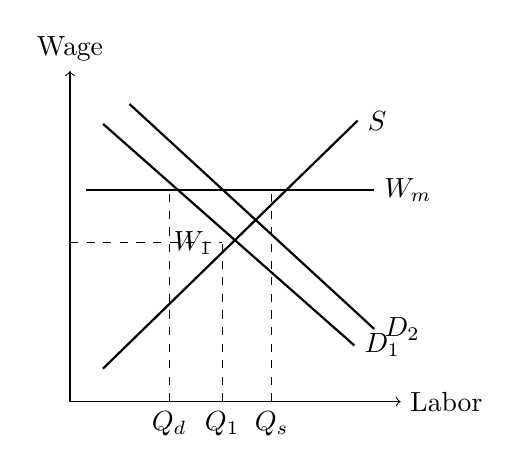
\begin{tikzpicture}[x=0.42cm,y=0.42cm]
\draw[->] (0,0) -- (10,0) node[right] {Labor};
\draw[->] (0,0) -- (0,10) node[above] {Wage};
\draw[thick] (1.0,1.0) -- (8.7,8.5) node[right] {$S$};
\draw[thick] (1.0,8.4) -- (8.6,1.7) node[right] {$D_1$};
\draw[thick] (1.8,9.0) -- (9.2,2.2) node[right] {$D_2$};
\draw[thick] (0.5,6.4) -- (9.2,6.4) node[right] {$W_m$};
\draw[dashed] (4.6,0) -- (4.6,4.8);
\draw[dashed] (3.0,0) -- (3.0,6.4);
\draw[dashed] (6.1,0) -- (6.1,6.4);
\draw[dashed] (0,4.8) -- (4.6,4.8) node[left] {$W_1$};
\node[below] at (4.6,0) {$Q_1$};
\node[below] at (3.0,0) {$Q_d$};
\node[below] at (6.1,0) {$Q_s$};
\end{tikzpicture}
\end{center}
\end{stimulus}
\begin{enumerate}[resume*=curveq, leftmargin=*, itemsep=0.8em, topsep=0.18em, parsep=0pt]
\item If worker productivity increases so that labor demand shifts from $D_1$ to $D_2$, the competitive equilibrium wage and employment will
\begin{choiceslist}
\item both decrease
\item both increase
\item wage will increase and employment will decrease
\item wage will decrease and employment will increase
\item remain unchanged because the labor supply curve does not shift
\end{choiceslist}
\item At the binding minimum wage $W_m$, employment and unemployment in this labor market are
\begin{choiceslist}
\item employment $Q_s$ and unemployment $Q_s-Q_d$
\item employment $Q_d$ and unemployment $Q_s-Q_d$
\item employment $Q_1$ and unemployment $Q_d-Q_1$
\item employment $Q_d$ and unemployment $Q_d-Q_s$
\item employment $Q_s$ and no unemployment because wage is above equilibrium
\end{choiceslist}
\item Total earnings received by workers who remain employed at the minimum wage are
\begin{choiceslist}
\item $W_1 \cdot Q_1$
\item $W_1 \cdot Q_d$
\item $W_m \cdot Q_d$
\item $W_m \cdot Q_s$
\item $W_m(Q_s-Q_d)$
\end{choiceslist}
\item A minimum wage like $W_m$ is more likely to increase the total earnings of labor when labor demand is
\begin{choiceslist}
\item relatively elastic
\item relatively inelastic
\item perfectly elastic
\item perfectly inelastic only
\item unit elastic
\end{choiceslist}
\end{enumerate}
\Needspace{18\baselineskip}
\begin{stimulus}
The following questions refer to the graph below, which shows a monopsonistic labor market.

\begin{center}
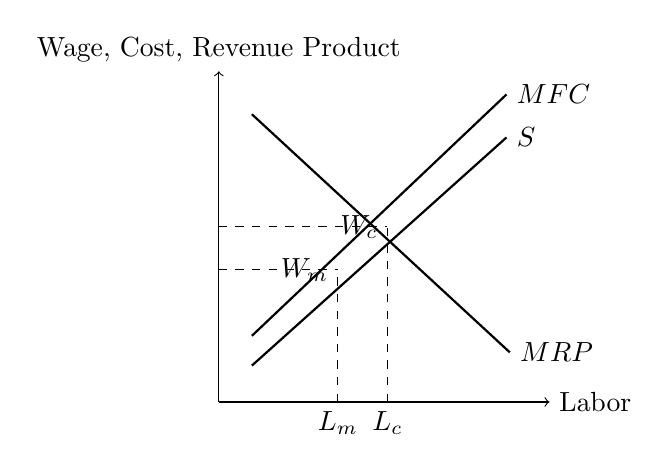
\begin{tikzpicture}[x=0.42cm,y=0.42cm]
\draw[->] (0,0) -- (10,0) node[right] {Labor};
\draw[->] (0,0) -- (0,10) node[above] {Wage, Cost, Revenue Product};
\draw[thick] (1.0,1.1) -- (8.7,8.0) node[right] {$S$};
\draw[thick] (1.0,2.0) -- (8.7,9.3) node[right] {$MFC$};
\draw[thick] (1.0,8.7) -- (8.8,1.5) node[right] {$MRP$};
\draw[dashed] (3.6,0) -- (3.6,4.0);
\draw[dashed] (5.1,0) -- (5.1,5.3);
\draw[dashed] (0,4.0) -- (3.6,4.0) node[left] {$W_m$};
\draw[dashed] (0,5.3) -- (5.1,5.3) node[left] {$W_c$};
\node[below] at (3.6,0) {$L_m$};
\node[below] at (5.1,0) {$L_c$};
\end{tikzpicture}
\end{center}
\end{stimulus}
\begin{enumerate}[resume*=curveq, leftmargin=*, itemsep=0.8em, topsep=0.18em, parsep=0pt]
\item In the unregulated monopsony, the firm will hire
\begin{choiceslist}
\item $L_c$ workers and pay wage $W_c$
\item $L_m$ workers and pay wage $W_m$
\item $L_m$ workers and pay wage $W_c$
\item $L_c$ workers and pay wage $W_m$
\item more than $L_c$ workers because $MFC$ exceeds $S$
\end{choiceslist}
\item Compared with a competitive labor market, the monopsony outcome results in
\begin{choiceslist}
\item higher wages and higher employment
\item higher wages and lower employment
\item lower wages and lower employment
\item lower wages and higher employment
\item the same wage but lower employment
\end{choiceslist}
\item If the government sets a minimum wage equal to $W_c$, the most likely result is that employment
\begin{choiceslist}
\item falls below $L_m$
\item remains at $L_m$
\item rises to $L_c$
\item rises above $L_c$
\item becomes zero because the wage is above $W_m$
\end{choiceslist}
\item The reason the $MFC$ curve lies above the labor supply curve is that
\begin{choiceslist}
\item the firm must pay a lower wage to inframarginal workers when it hires another worker
\item the firm can only hire labor if it also hires more capital
\item hiring an additional worker requires raising the wage paid to all workers
\item the labor supply curve is downward sloping to the firm
\item marginal revenue product rises faster than wage
\end{choiceslist}
\end{enumerate}
\Needspace{18\baselineskip}
\begin{stimulus}
The following questions refer to the graph below, which shows a market generating a negative production externality.

\begin{center}
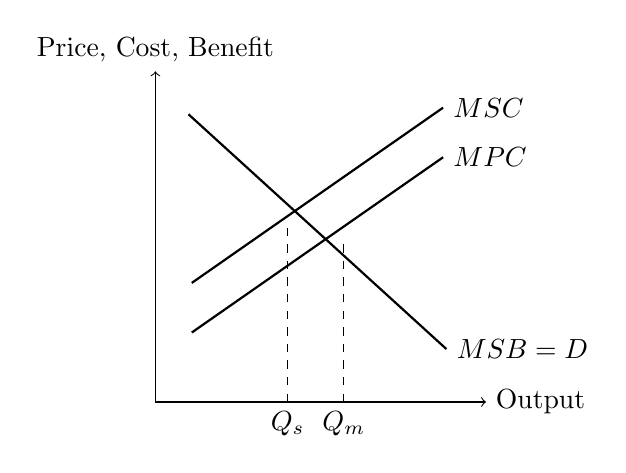
\begin{tikzpicture}[x=0.42cm,y=0.42cm]
\draw[->] (0,0) -- (10,0) node[right] {Output};
\draw[->] (0,0) -- (0,10) node[above] {Price, Cost, Benefit};
\draw[thick] (1.0,8.7) -- (8.8,1.6) node[right] {$MSB=D$};
\draw[thick] (1.1,2.1) -- (8.7,7.4) node[right] {$MPC$};
\draw[thick] (1.1,3.6) -- (8.7,8.9) node[right] {$MSC$};
\draw[dashed] (4.0,0) -- (4.0,5.4);
\draw[dashed] (5.7,0) -- (5.7,4.9);
\node[below] at (4.0,0) {$Q_s$};
\node[below] at (5.7,0) {$Q_m$};
\end{tikzpicture}
\end{center}
\end{stimulus}
\begin{enumerate}[resume*=curveq, leftmargin=*, itemsep=0.8em, topsep=0.18em, parsep=0pt]
\item The unregulated market quantity is
\begin{choiceslist}
\item $Q_s$, because the market accounts for all costs
\item $Q_s$, because $MSB$ intersects $MSC$ there
\item $Q_m$, because private decision makers equate marginal private cost with demand
\item $Q_m$, because marginal social cost is below marginal private cost
\item indeterminate because no prices are labeled
\end{choiceslist}
\item A per-unit Pigouvian tax that corrects the externality should be equal to
\begin{choiceslist}
\item the vertical distance between $MSB$ and $MPC$ at $Q_m$
\item the vertical distance between $MSC$ and $MPC$ at $Q_s$
\item the horizontal distance between $Q_m$ and $Q_s$
\item the vertical distance between $MSB$ and $MSC$ at $Q_s$
\item the entire deadweight loss triangle
\end{choiceslist}
\item The deadweight loss from the unregulated market is the area
\begin{choiceslist}
\item between $MSB$ and $MPC$ from 0 to $Q_s$
\item between $MSC$ and $MPC$ from 0 to $Q_s$
\item between $MSC$ and $MSB$ from $Q_s$ to $Q_m$
\item between $MSB$ and $MPC$ from $Q_s$ to $Q_m$
\item between $MSC$ and $MPC$ from $Q_s$ to $Q_m$ plus the rectangle below it
\end{choiceslist}
\item If the government successfully imposes the corrective tax, which of the following will most likely occur?
\begin{choiceslist}
\item Output will rise from $Q_m$ to $Q_s$ and total surplus will fall.
\item Output will fall from $Q_m$ to $Q_s$ and total surplus will rise.
\item Output will fall below $Q_s$ and total surplus will fall.
\item Output will remain at $Q_m$ and firms will simply earn lower profit.
\item Output will rise above $Q_m$ because tax revenue funds public goods.
\end{choiceslist}
\end{enumerate}
\Needspace{18\baselineskip}
\begin{stimulus}
The following questions refer to the Lorenz-curve graph below.

\begin{center}
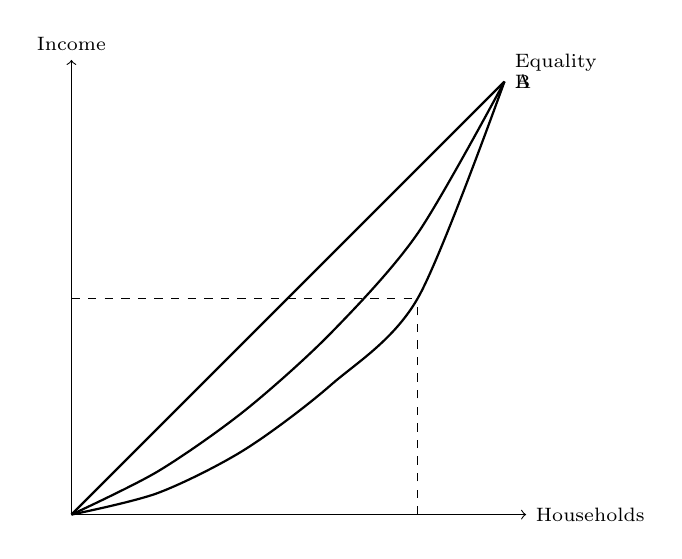
\begin{tikzpicture}[x=0.055cm,y=0.055cm]
\draw[->] (0,0) -- (105,0) node[right] {\scriptsize Households};
\draw[->] (0,0) -- (0,105) node[above] {\scriptsize Income};
\draw[thick] (0,0) -- (100,100) node[above right] {\scriptsize Equality};
\draw[thick] plot[smooth] coordinates {(0,0) (20,5) (40,15) (60,30) (80,50) (100,100)} node[right] {\scriptsize A};
\draw[thick] plot[smooth] coordinates {(0,0) (20,10) (40,24) (60,42) (80,65) (100,100)} node[right] {\scriptsize B};
\draw[dashed] (80,0) -- (80,50);
\draw[dashed] (0,50) -- (80,50);
\end{tikzpicture}
\end{center}
\end{stimulus}
\begin{enumerate}[resume*=curveq, leftmargin=*, itemsep=0.8em, topsep=0.18em, parsep=0pt]
\item Based on the graph, which country has the more equal distribution of income?
\begin{choiceslist}
\item Country A, because its Lorenz curve lies farther from the line of equality
\item Country A, because its top 20\% receives a smaller share of income
\item Country B, because its Lorenz curve lies closer to the line of equality
\item Country B, because its Lorenz curve is steeper near the origin
\item The two countries are equally distributed because both end at 100\%, 100\%
\end{choiceslist}
\item Which of the following is true about the Gini coefficients of the two countries?
\begin{choiceslist}
\item Country A has the smaller Gini coefficient.
\item Country B has the smaller Gini coefficient.
\item They must be equal because both countries have a Lorenz curve.
\item Country B's Gini coefficient must exceed 1.
\item The Gini coefficient cannot be related to a Lorenz curve.
\end{choiceslist}
\item A progressive tax-and-transfer system that reduces inequality would most likely shift a country's Lorenz curve
\begin{choiceslist}
\item away from the line of equality
\item toward the line of equality
\item downward only at the 100\% endpoint
\item into a perfectly horizontal line
\item into a perfectly vertical line
\end{choiceslist}
\item In Country A, the graph shows that the bottom 80\% of households receive 50\% of total income. Therefore, the top 20\% of households receive
\begin{choiceslist}
\item 20\% of total income
\item 30\% of total income
\item 40\% of total income
\item 50\% of total income
\item 80\% of total income
\end{choiceslist}
\end{enumerate}
\end{multicols*}
\label{LastPage}
\end{document}
